\documentclass{article}
\usepackage{graphicx}
\usepackage{amsmath}
\usepackage{minted}
\usepackage{subcaption}
\usepackage{listings}
\usepackage{hyperref}

\title{Differential Equations Coding Project}
\author{Cam Walter}
\date{April 24, 2024}

\begin{document}

\maketitle

\section{Questions}
\begin{enumerate}
      \item
            \begin{enumerate}
                  \item \begin{math}
                              f(x) = -5 + 0.5x^2 + x^5
                        \end{math}
                  \item The solution would not work, since we would need a degree 6
                        polynomial now. This makes sense, since if we added a row to multiply,
                        there would not be enough columns in \textit{A} to match up with \textit{x}'s rows.
                  \item \begin{math}
                              det(V)=0 \iff \exists x_i, x_j (x_i=x_j, i \neq j)
                        \end{math}
                        \begin{figure}[h]
                              \centering
                              \begin{subfigure}{.5\textwidth}
                                    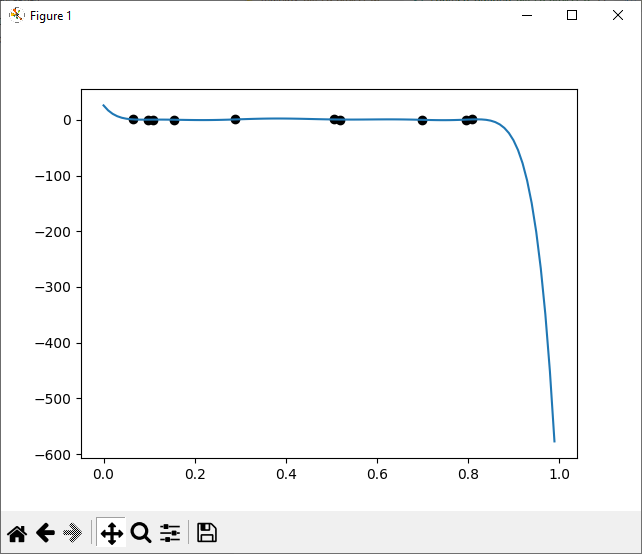
\includegraphics[width=\textwidth, keepaspectratio]{zoomed_out.png}
                              \end{subfigure}\hfill
                              \begin{subfigure}{.5\textwidth}
                                    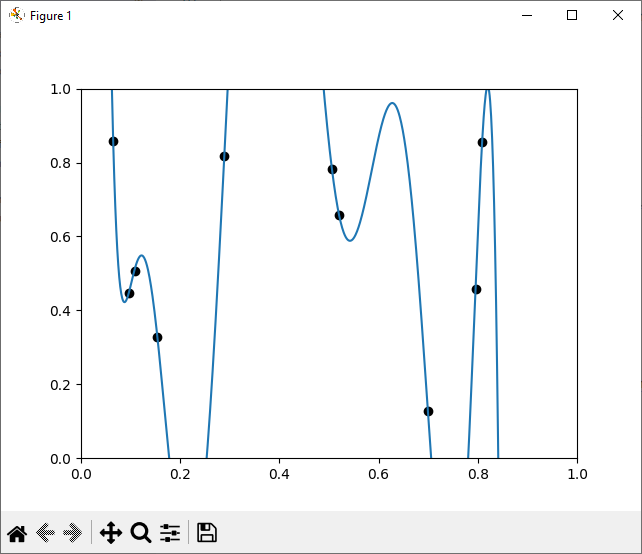
\includegraphics[width=\textwidth, keepaspectratio]{zoomed_in.png}
                              \end{subfigure}

                              \caption{Zoomed out and in views of the data set}
                              \label{graph:1}
                        \end{figure}
                  \item See \autoref{graph:1} and \autoref{points}.
                  \item We can use spline interpretation to form a piecewise function
                        comprised ofseveral small polynomials to make the graph much better
                        reflect the data points.
            \end{enumerate}

      \item \begin{enumerate}
                  \item \begin{math}
                              \lambda_1=5.652811297306327
                        \end{math}
                  \item \begin{math}
                              \lambda_2=1.3215412408013711
                        \end{math}
            \end{enumerate}
\end{enumerate}

\pagebreak

\section{Code}
\inputminted{python3}{main.py}

\section{Points} \label{points}
\lstinputlisting{points.txt}

\end{document}
